\documentclass{beamer}
\mode<presentation>
\usepackage{amsmath,amssymb,mathtools}
\usepackage{textcomp}
\usepackage{gensymb}
\usepackage{adjustbox}
\usepackage{subcaption}
\usepackage{enumitem}
\usepackage{multicol}
\usepackage{listings}
\usepackage{url}
\usepackage{graphicx} % <-- needed for images
\def\UrlBreaks{\do\/\do-}

\usetheme{Boadilla}
\usecolortheme{lily}
\setbeamertemplate{footline}{
  \leavevmode%
  \hbox{%
  \begin{beamercolorbox}[wd=\paperwidth,ht=2ex,dp=1ex,right]{author in head/foot}%
    \insertframenumber{} / \inserttotalframenumber\hspace*{2ex}
  \end{beamercolorbox}}%
  \vskip0pt%
}
\setbeamertemplate{navigation symbols}{}

\lstset{
  frame=single,
  breaklines=true,
  columns=fullflexible,
  basicstyle=\ttfamily\tiny   % tiny font so code fits
}

\numberwithin{equation}{section}

% ---- your macros ----
\providecommand{\nCr}[2]{\,^{#1}C_{#2}}
\providecommand{\nPr}[2]{\,^{#1}P_{#2}}
\providecommand{\mbf}{\mathbf}
\providecommand{\pr}[1]{\ensuremath{\Pr\left(#1\right)}}
\providecommand{\qfunc}[1]{\ensuremath{Q\left(#1\right)}}
\providecommand{\sbrak}[1]{\ensuremath{{}\left[#1\right]}}
\providecommand{\lsbrak}[1]{\ensuremath{{}\left[#1\right.}}
\providecommand{\rsbrak}[1]{\ensuremath{\left.#1\right]}}
\providecommand{\brak}[1]{\ensuremath{\left(#1\right)}}
\providecommand{\lbrak}[1]{\ensuremath{\left(#1\right.}}
\providecommand{\rbrak}[1]{\ensuremath{\left.#1\right)}}
\providecommand{\cbrak}[1]{\ensuremath{\left\{#1\right\}}}
\providecommand{\lcbrak}[1]{\ensuremath{\left\{#1\right.}}
\providecommand{\rcbrak}[1]{\ensuremath{\left.#1\right\}}}
\theoremstyle{remark}
\newtheorem{rem}{Remark}
\newcommand{\sgn}{\mathop{\mathrm{sgn}}}
\providecommand{\abs}[1]{\left\vert#1\right\vert}
\providecommand{\res}[1]{\Res\displaylimits_{#1}}
\providecommand{\norm}[1]{\lVert#1\rVert}
\providecommand{\mtx}[1]{\mathbf{#1}}
\providecommand{\mean}[1]{E\left[ #1 \right]}
\providecommand{\fourier}{\overset{\mathcal{F}}{ \rightleftharpoons}}
\providecommand{\system}{\overset{\mathcal{H}}{ \longleftrightarrow}}
\providecommand{\dec}[2]{\ensuremath{\overset{#1}{\underset{#2}{\gtrless}}}}
\newcommand{\myvec}[1]{\ensuremath{\begin{pmatrix}#1\end{pmatrix}}}
\let\vec\mathbf

\title{Matgeo Presentation - Problem 2.9.20}
\author{ai25btech11004 - Jaswanth}

\begin{document}


\frame{\titlepage}
\begin{frame}{Question}
$\vec{X}$ and  $\vec{Y}$ are two points with position vectors $3\vec{a}$+$\vec{b}$  and  $\vec{a}$-$3\vec{b}$, respectively. Write the position vector of a point Z  which divides the line segment  $\vec{XY}$ in the ratio 2:1 externally.\\
\end{frame}
\begin{frame}{solution}
\begin{align}
    \vec{X} &= 3\vec{a}+\vec{b}\\
    \vec{Y} &= \vec{a}-3\vec{b}
\end{align}

Now, the matrix form for $\vec{Y}$ and $\vec{X}$ is:
\begin{align}
\myvec{\vec{Y} & \vec{X}}
=\myvec{\vec{a} & \vec{b}}
\myvec{1 & 3 \\ -3 & 1}
\end{align}

Using the section formula, the point $\vec{Z}$ dividing $\vec{Y} - \vec{X}$ in ratio $2:1$ externally is:
\begin{align}
\vec{Z} &= \frac{2\vec{Y} - \vec{X}}{2-1} \\
\vec{Z} &=  \myvec{\vec{Y} & \vec{X}} \myvec{2 \\ -1} \\
\vec{Z} &=  \myvec{\vec{a} & \vec{b}}\myvec{1 & 3 \\ -3 & 1} \myvec{2 \\ -1} \end{align}
\end{frame}
\begin{frame}{solution}
\begin{align}
\vec{Z} &= \myvec{\vec{a} & \vec{b}} \myvec{-1 \\ -7} \\
\vec{Z} &= -\vec{a}-7\vec{b}  
\end{align}

\end{frame}
\begin{frame}{Plot}
    \begin{figure}[H]
    \centering
    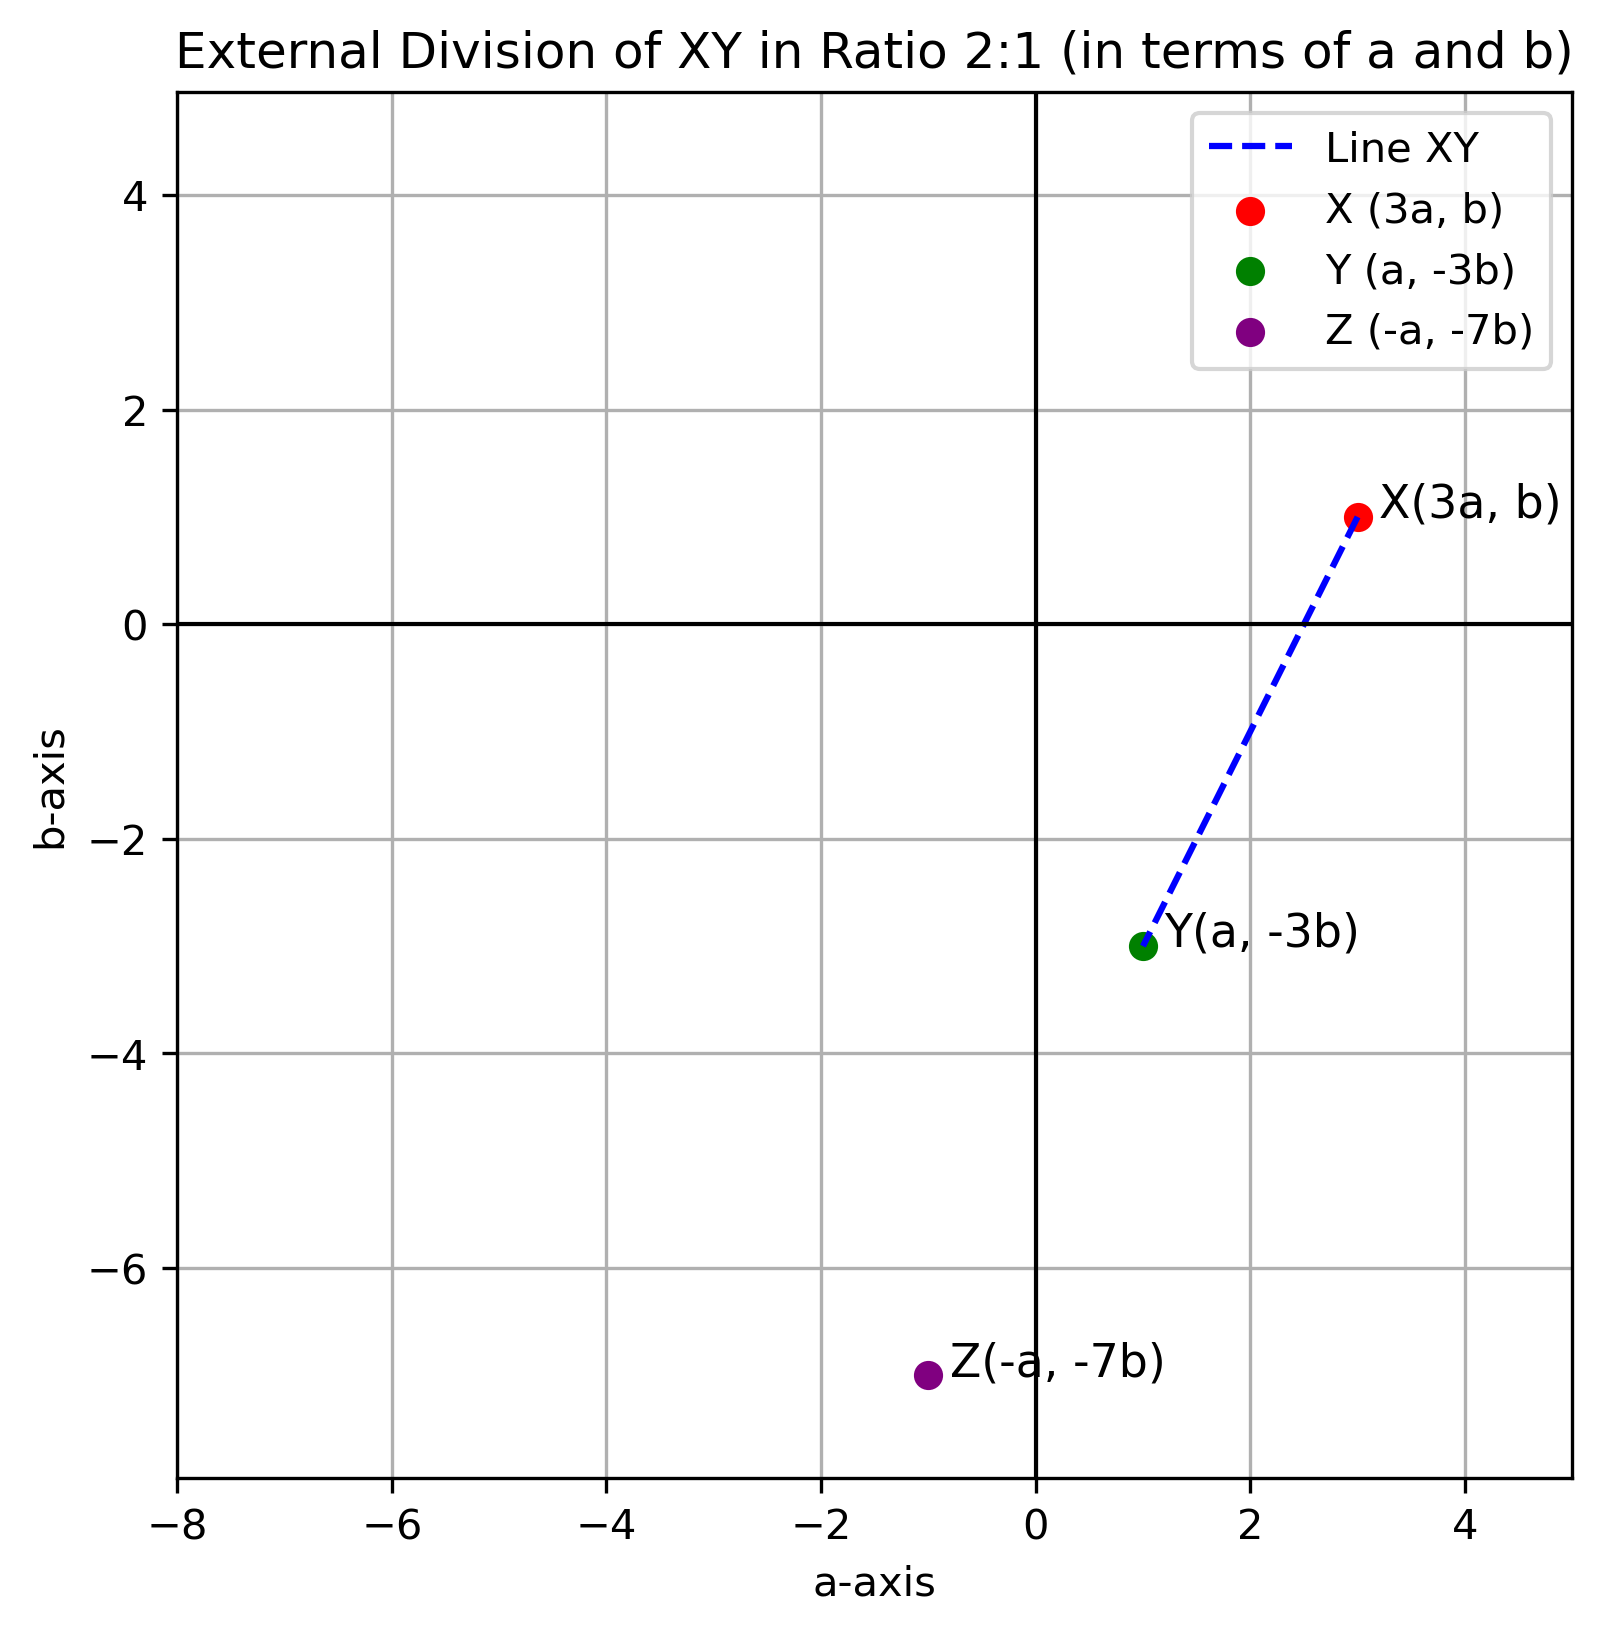
\includegraphics[width=0.71\columnwidth]{figs/01.png}
    \label{fig-1}
\end{figure}
\end{frame}

% --------- CODE APPENDIX ---------
\section*{Appendix: Code}

% C program
\begin{frame}[fragile]{C Code: Code.c}
\begin{lstlisting}[language=C]
#include <stdio.h>

int main() {
    FILE *fp;
    float a, b;
    float X1, X2, Y1, Y2, Z1, Z2;
    int k = 2;  // Ratio 2:1 (external division)

    // Input a and b
    printf("Enter values of a and b: ");
    scanf("%f %f", &a, &b);

    // Position vectors
    X1 = 3 * a;
    X2 = b;
    Y1 = a;
    Y2 = -3 * b;

    // External division formula: Z = (kY - X) / (k - 1)
    Z1 = (k * Y1 - X1) / (k - 1);
    Z2 = (k * Y2 - X2) / (k - 1);

    // Open file to write output
    fp = fopen("solution.dat", "w");
    if (fp == NULL) {
        printf("Error opening file!\n");
        return 1;
    }
 \end{lstlisting}
\end{frame}

\begin{frame}[fragile]{C Code: Code.c}
\begin{lstlisting}[language=C]
    // Write result to file
    fprintf(fp, "External Division of XY in ratio 2:1\n");
    fprintf(fp, "Given:\n");
    fprintf(fp, "X = (3a, b)\nY = (a, -3b)\n");
    fprintf(fp, "Computed position vector of Z:\n");
    fprintf(fp, "Z = (%.2fa, %.2fb)\n", Z1/a, Z2/b); // symbolic form
    fprintf(fp, "Or numerically: (%.2f, %.2f)\n", Z1, Z2);

    fclose(fp);

    printf(" Output written to 'solution.dat'\n");
    return 0;
}


    \end{lstlisting}
\end{frame}
\begin{frame}[fragile]{Python: plot.py}
\begin{lstlisting}[language=Python]
  import numpy as np
import matplotlib.pyplot as plt

# Symbolic vectors (set a = 1, b = 1 for proportional plotting)
a, b = 1, 1

# Given position vectors
X = np.array([3*a, b])      # (3a, b)
Y = np.array([a, -3*b])     # (a, -3b)
k = 2                       # ratio 2:1 externally

# External division formula: Z = (kY - X) / (k - 1)
Z = (k*Y - X) / (k - 1)     # should give (-a, -7b)

# Plot
plt.figure(figsize=(6,6))
plt.plot([X[0], Y[0]], [X[1], Y[1]], 'b--', label='Line XY')
plt.scatter(*X, color='red', label='X (3a, b)')
plt.scatter(*Y, color='green', label='Y (a, -3b)')
plt.scatter(*Z, color='purple', label='Z (-a, -7b)')

# Annotate points
plt.text(X[0]+0.2, X[1], 'X(3a, b)', fontsize=11)
plt.text(Y[0]+0.2, Y[1], 'Y(a, -3b)', fontsize=11)
plt.text(Z[0]+0.2, Z[1], 'Z(-a, -7b)', fontsize=11)

# Axes styling
plt.axhline(0, color='black', linewidth=1)
plt.axvline(0, color='black', linewidth=1)
plt.grid(True)
plt.axis('equal')
plt.xlim(-8, 5)
plt.ylim(-8, 5)
\end{lstlisting}
\end{frame}
\begin{frame}[fragile]{Python: plot.py}
\begin{lstlisting}[language=Python]
plt.xlabel('a-axis')
plt.ylabel('b-axis')
plt.title('External Division of XY in Ratio 2:1 (in terms of a and b)')
plt.legend()

# Save figure
plt.savefig("external_division.png", dpi=300, bbox_inches='tight')
plt.show()

print("✅ Figure saved as 'external_division.png'")

\end{lstlisting}
\end{frame}

\end{document}
